\chapter{User manual}\label{sec:user_manual}
We have written a manual for people who want to recreate our demonstration. The demonstration could for example be shown off at exhibitions. The manual could also be used for people who want to further test and develop our IoT-system.

First check the IP-address of the internet you are connected to, and the usable ports. Make sure that your computer hosting the server and the vehicles are connected to the same network.

\begin{lstlisting}
$ipconfig getifaddr en0
192.168.56.208
\end{lstlisting}

Then open the Server solution in your code editor, we have used visual studio. Under the folder “properties” there is a file called launchSettings.json. In that file write in the ip address and the port in the applicationUrl-section:

\begin{json}
"profiles": {
	"SignalRServer": {
		"commandName": "Project",
		"dotnetRunMessages": true,
		"launchBrowser": false,
		"applicationUrl": "https://192.168.56.208:7058;http://192.168.56.208:5048",
		"environmentVariables": {
			"ASPNETCORE_ENVIRONMENT": "Development"
		}
	},
\end{json}
	
After that, open the Client solution. Here we used Pycharm as the IDE. Open the config.json document and replace the same IP address and port:
	
\begin{json}
"client": {
	"host": "192.168.56.208",
	"port": 5048,
	"delay": 0.1
},
\end{json}
	
	If the vehicles have not connected to that network before, they need to log on to that network. To log on to a new network; connect the Raspberry Pi to a power source and a display, and use the user interface. The display port on the Raspberry Pi is a micro USB port. When the Raspberry Pi has booted up, click on the internet icon and connect to the same network as the server. If the network has been connected to it before, Raspberry Pi will automatically connect to that network during boot up.
	
	The initial speed of the vehicles can be changed by adjusting the value of \verb|SpeedLimit| located at VehicleHubDatabase under the Database folder on the server solution:
\begin{csharp}
public class VehiclesHubDatabase : IVehiclesHubDatabase
{
	...
	public double SpeedLimit => 80;
	...
}
\end{csharp}
Moreover, the configuration of the road can also be changed by changing the following section of the code:
\begin{csharp}
public class VehiclesHubDatabase : IVehiclesHubDatabase
{
	...
	public VehiclesHubDatabase()
	{
		_intersection = new Intersection().
			AddRoad(new Road {Length = 300}.
				AddLane(null, true).
				AddLane()).
			AddRoad(new Road {Length = 300}.
				AddLane(null, true).
				AddLane());
		...
	}
	...
}
\end{csharp}
The current configuration shown above corresponds to the same configuration shown in \figref{fig:intersectionconcept}. The intersection can be moved by adding additional arguments such as:
\begin{csharp}
	public class VehiclesHubDatabase : IVehiclesHubDatabase
	{
		...
		public VehiclesHubDatabase()
		{
			_intersection = new Intersection().
				AddRoad(new Road {Length = 300}.
					AddLane(null, true).
					AddLane(), 200).
				AddRoad(new Road {Length = 300}.
					AddLane(null, true).
					AddLane(), 150);
			...
		}
		...
	}
\end{csharp}
\figref{fig:altintersectionconfig} shows the resulting topology by adding extra parameters to the code above.
\begin{figure}[h!]
	\centering
	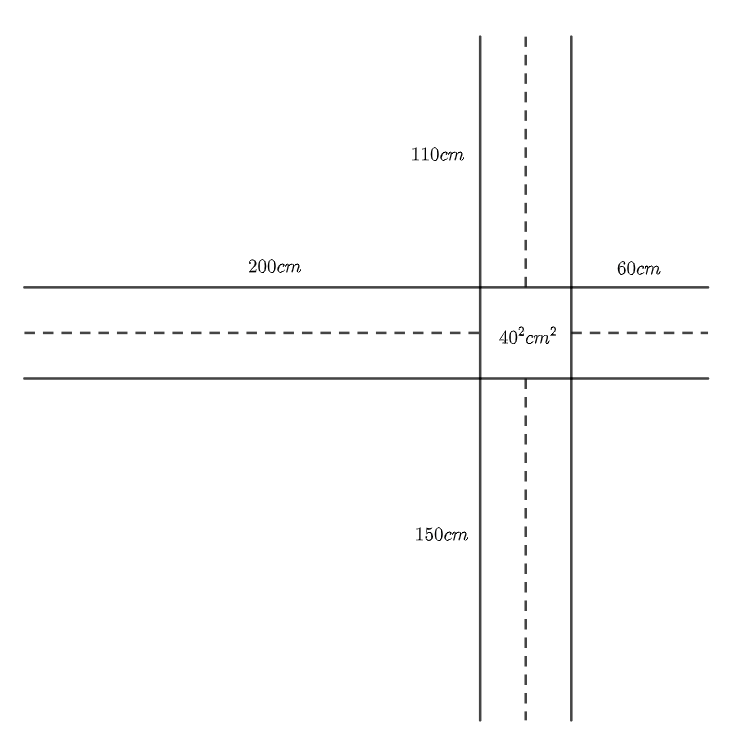
\includegraphics[width=1\linewidth]{figures/alt_intersection_config}
	\caption{An alternative configuration of the intersection and its connected roads by adding extra parameter to the initialization of the intersection as described by the previous code snippet.}
	\label{fig:altintersectionconfig}
\end{figure}

The length is in centimeters and needs to correlate with the length of the physical track. We used tape to show where the roads were. However, this is unnecessary. We recommend a track between three to four meters long for the best results.

Lastly, position both vehicles down at the start of the two tracks, turn on the server and connect to the power banks. The vehicles should automatically connect to the server after 20-30 seconds. When both vehicles have established a connection to the server, the demonstration has started.